\documentclass[handout]{beamer}

\usepackage{Vor2018glærur}

\title{Tölvunarfræði 2}
\subtitle{Vika 2}

\begin{document}

\begin{frame}
\titlepage
\end{frame}

\section{Breytur og minni í C++}

\begin{frame}{Líftími breyta}
\begin{itemize}
 \item Við munum að breytur hafa mismunandi líftíma
 \begin{itemize}
  \item Aðskilið hugtak: gildissvið breytu (e. \emph{variable scope})
 \end{itemize}
 \item Í C++ getur líftími breytu verið af nokkrum gerðum, þá helst
 \begin{itemize}
  \item Sjálfvirkur (e. \emph{automatic}) - líftími breytunnar er ákvarðaður sjálfkrafa
  \item Kyrrstæður (e. \emph{static}) - breytan lifir meðan forritið keyrir
  \item Kvikstæður (e. \emph{dynamic}) - breytan lifir meðan forritari segir
 \end{itemize}
 \item Í flestum forritunarmálum sem við erum líkleg til að hafa skoðað hingað til sér ruslasafnari (e. \emph{garbage collector}) um að hreinsa til, en venjulegt C++ hefur ekki slíkan
\end{itemize}
\end{frame}

\begin{frame}{Minnissvæði í C++}
\begin{itemize}
 \item Í keyrandi C++ forriti eru (venjulega) nokkrar gerðir minnis í gangi á hverjum tímapunkti
 \begin{itemize}
  \item Þula (e. \emph{code segment}). Geymir upplýsingar um forritið - vélamálsskipanir og fasta, venjulega er eingöngu lesaðgangur
  \item Gagnasvæði (e. \emph{data segment}).
  Frátekið í upphafi keyrslu, getum ekki stækkað eða minnkað.
  \item Hlaði (e. \emph{stack}). Minnissvæði af breytilegri stærð sem hægt er að fá aðgang að á skipulegan máta
  \item Kös (e. \emph{heap}). Er úthlutað og skilað að beiðni forritsins, minnisdreifing ekki endilega mjög fyrirsjáanleg
 \end{itemize}
 \item Hlaðinn og kösin eru þau svæði sem við þurfum að skoða sérstaklega
\end{itemize}
\end{frame}

\begin{frame}{Hvað fer svo hvert?}
\begin{itemize}
 \item Þumalputtareglur fyrir ``venjulegt'' C++
 \begin{itemize}
  \item Líftími staðværra (e. \emph{local}) breyta er ákvarðaður sjálfkrafa og þær eru settar á hlaðann
  \item Víðværar (e. \emph{global}) breytur og breytur skilgreindar sem \texttt{static} fara í gagnasvæðið
  \item Kvikstæðar breytur fást með sérstökum minnisúthlutunaraðgerðum eins og \texttt{new} og eru settar í kös
 \end{itemize}
\end{itemize}
\end{frame}

\begin{frame}{Hlaðinn}
\begin{columns}
\column{0.6\textwidth}
\begin{itemize}
 \item Hlaðinn er ``lítið'' minnissvæði sem C++ forrit nota til að halda utan um staðværar breytur og upplýsingar um fallsköll
 \begin{itemize}
  \item Getum lent í því að hlaðinn fyllist
 \end{itemize}
 \item Uppbygging er skipuleg (LIFO)
 \begin{itemize}
  \item Hentar vel fyrir raunverulega örgjörva, gerir mjög hraða vinnslu mögulega
 \end{itemize}
 \item Líftíma breyta á hlaðanum er stjórnað sjálfkrafa í C++, minninu er skilað þegar viðkomandi fall skilar af sér
\end{itemize}
\column{0.4\textwidth}
\begin{center}
Uppbygging hlaðans

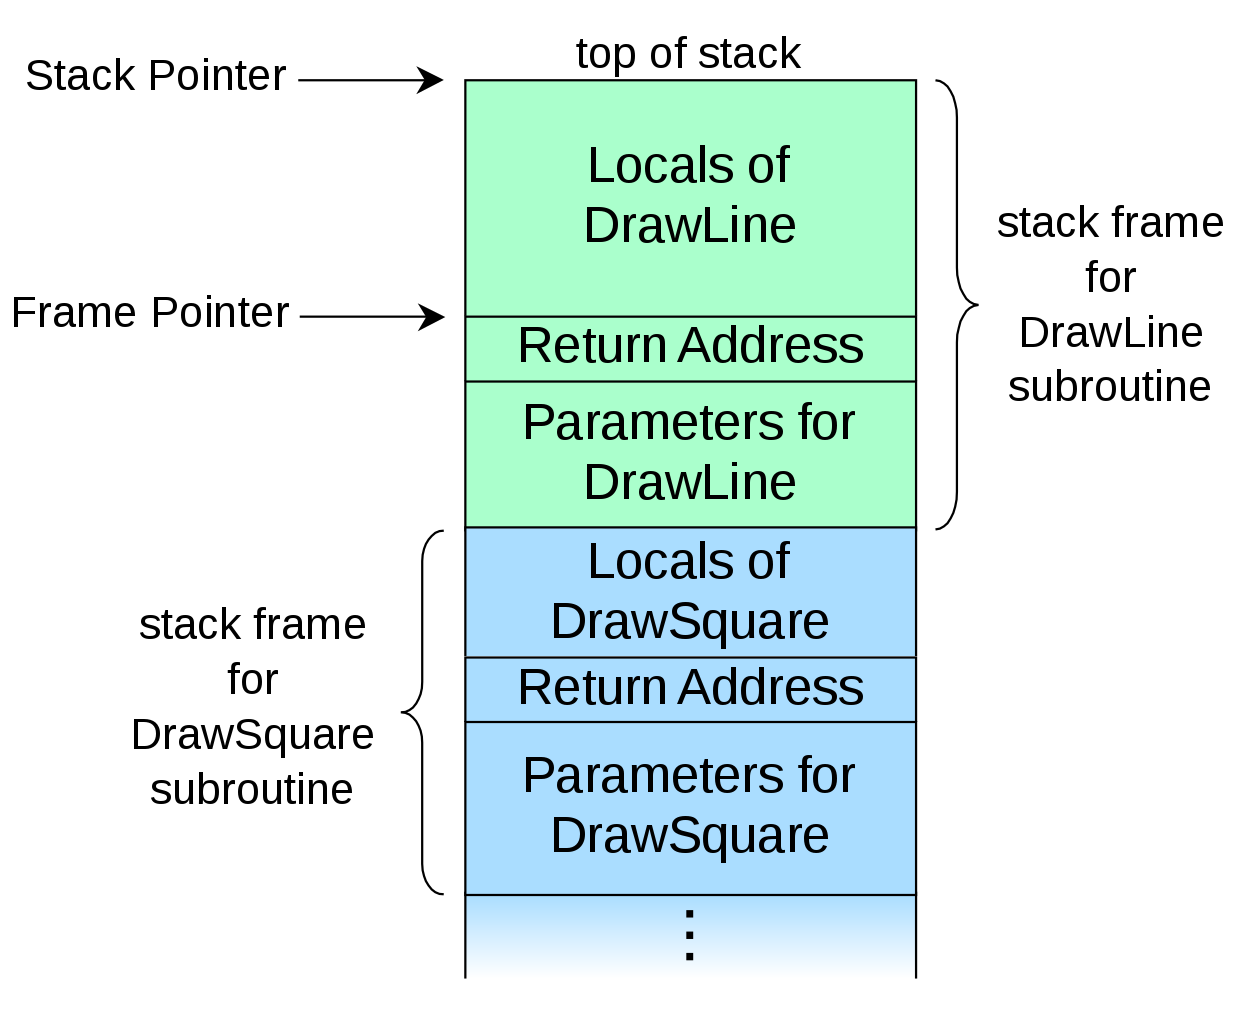
\includegraphics[width=\linewidth]{call-stack-layout}

{\tiny Mynd: \href{https://en.wikipedia.org/wiki/File:Call_stack_layout.svg}{Wikimedia}}
\end{center}
\end{columns}
\end{frame}

\begin{frame}{Kösin}
\begin{columns}
\column{0.7\textwidth}
\begin{itemize}
 \item Kösin er ``stórt'' minnissvæði sem C++ forrit geta beðið um skerf af á keyrslutíma
 \item Er ekki endilega samfellt, getur verið mjög uppskipt (e. \emph{fragmented})
 \item Hægur aðgangur í samanburði við aðgang að hlaðanum
 \item Hægt er að fá aðgang að kösinni hvaðan sem er úr forritinu
 \begin{itemize}
  \item Takmarkast ekki við fallskall
 \end{itemize}
 \item C++ forrit sem fær aðgang að kös með \texttt{new} þarf að skila svæðinu með \texttt{delete}
\end{itemize}
\column{0.3\textwidth}
\begin{center}
Vond uppskipting

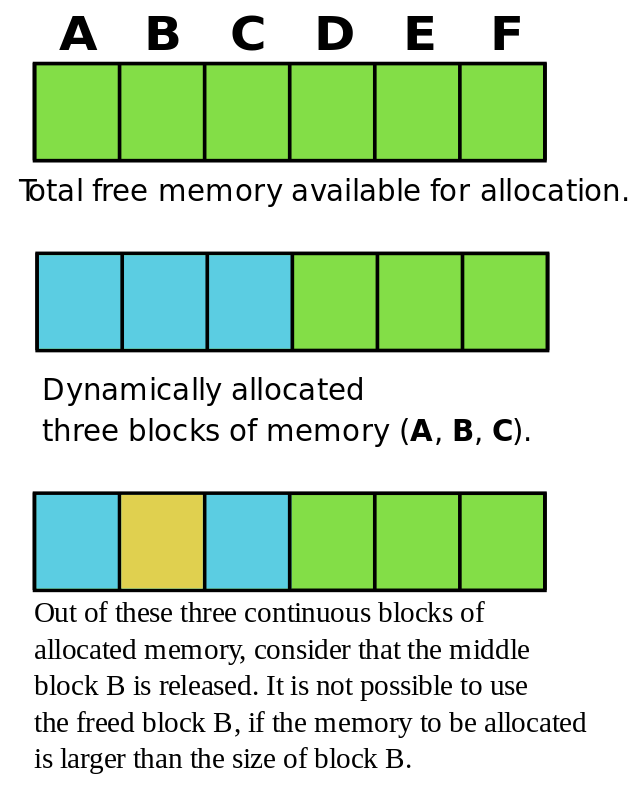
\includegraphics[width=\linewidth]{external-fragmentation}

{\tiny Mynd: \href{https://commons.wikimedia.org/wiki/File:External_Fragmentation.svg}{Wikimedia}}
\end{center}
\end{columns}
\end{frame}

\subsection{Upprifjun á bendum}

\begin{frame}{Bendar}
\begin{itemize}
 \item Bendir er breyta sem inniheldur staðsetningu minnissvæðis
 \begin{itemize}
  \item Hún ``bendir á'' minnissvæðið
 \end{itemize}
 \item Hægt er að nota bendinn til að fá aðgang að gögnunum sem geymd eru í minnissvæðinu
 \begin{itemize}
  \item {\color{red} Nýtt}: Gagnlegt þegar gögnin eru í kös!
 \end{itemize}
\end{itemize}
\begin{center}
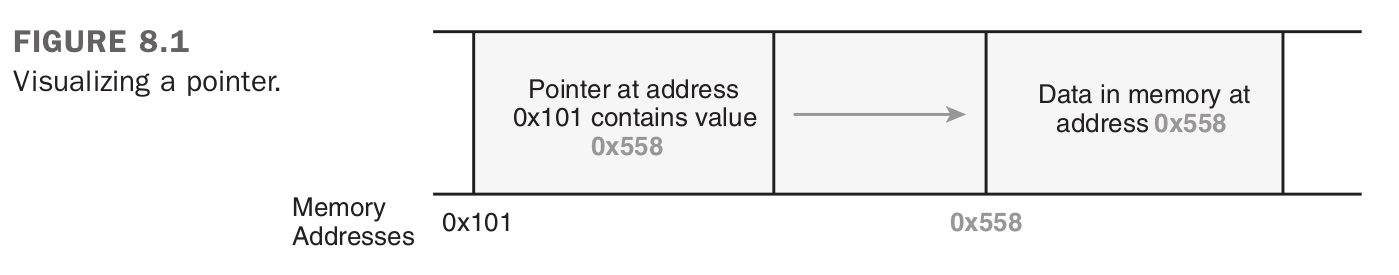
\includegraphics[width=\textwidth]{pointer-visualization}
\end{center}
\end{frame}

\begin{frame}[fragile]{Bendar}
Við getum búið til bendi sem vísar á breytu af gerðinni \texttt{gerd} með \texttt{gerd*}, náð í  staðsetningu minnissvæðis með \texttt{\&} virkjanum og sótt gögn sem bendir vísar á með \texttt{*} virkjanum

\cppfile[firstline=6, lastline=15, gobble=4, fontsize=\small, label=dereferencing.cpp]{Code/w1/dereferencing.cpp}
\end{frame}

\begin{frame}[fragile]{Nýtt trix}
Nýtt trix: Notum \texttt{new} til að taka frá minnissvæði í kös fyrir breytu og skila bendi á minnissvæðið.
\begin{minted}[fontsize=\small, frame=lines]{cpp}
// request memory for one element
Type* pointer = new Type;
// request memory for numElements
Type* pointer = new Type[numElements];
\end{minted}
Til að taka frá minni í kös fyrir heiltölur:
\begin{minted}[fontsize=\small, frame=lines]{cpp}
// get a pointer to an integer
int* pointToAnInt = new int;
// pointer to a block of 10 integers
int* pointToNums = new int[10];
\end{minted}
\end{frame}

\begin{frame}[fragile]{new og delete}

\cppfile[firstline=11, lastline=18, gobble=4, fontsize=\small, label=dynamicdouble.cpp]{Code/w2/dynamicdouble.cpp}

\end{frame}

\subsection{Föll og breytur}

\begin{frame}{Föll og breytur í C++}
\begin{itemize}
 \item Við höfum töluverða stjórn á hvernig C++ meðhöndlar inntaksbreytur og skilabreytur
 \item Sjálfgefið er að C++ noti gildisviðföng (e. \emph{value passing})
 \begin{itemize}
  \item En stundum er það ekki skilvirkt
  \item Stundum er það það ekki mögulegt
 \end{itemize}
 \item Annar möguleiki: Taka inn og skila bendum
\end{itemize}
\end{frame}

\begin{frame}{Meira um fylki í C++}
Munum: ``gamaldags'' fylki í C++ eru þunn skel utan um benda.

\cppfile[firstline=6, lastline=9, gobble=4, label=arraysandpointers.cpp]{Code/w2/arraysandpointers.cpp}
Þetta setur takmarkanir á hvernig hægt er að nota fylki sem inntaks- og úttaksbreytur.
\end{frame}

\begin{frame}{Fylki sem bendar}
Tvær leiðir til að skrifa út stökin sem eru í þriggja staka fylkinu \texttt{pizzaSizes}
\begin{columns}
\column{0.45\textwidth}
\cppfile[firstline=10, lastline=17, gobble=4, label=arraysandpointers.cpp, fontsize=\scriptsize, linenos=false]{Code/w2/arraysandpointers.cpp}
\column{0.55\textwidth}
\cppfile[firstline=22, lastline=27, gobble=4, label=arraysandpointers.cpp, fontsize=\scriptsize, linenos=false]{Code/w2/arraysandpointers.cpp}
\end{columns}
\end{frame}

\section{Hlutbundin forritun í C++}

\begin{frame}{Hlutbundin forritun}
\begin{itemize}
 \item Ein aðalástæðan fyrir því að C++ var búið til er að forritunarmálið C styður ekki hlutbundna forritun
 \item Hlutbundin forritun hefur ýmsar birtingarmyndir, en í C++ og málum sem á eftir koma höfum við:
 \begin{itemize}
  \item Hlutir (e. \emph{objects}) - grundvallareiningin í hlutbundinni forritun
  \begin{itemize}
   \item Hlutur er ``pakki'' af gögnum og aðgerðum á gögnin
  \end{itemize}
  \item Klasar (e. \emph{classes}) eru notaðir til að skilgreina ``gerð'' af hlutum 
 \end{itemize}
 \item Tölum um að hlutur sé tilvik (e. \emph{instance}) af klasa
 \item Getum litið á það sem svo að hlutbundin forritun sé leið okkar til að bæta við tögunarkerfi málsins
\end{itemize}
\end{frame}

\begin{frame}{Dæmi um klasa}
Klasi sem táknar mannveru og \texttt{main} fall sem býr til tilvik.
\begin{columns}
\column{0.45\textwidth}
\cppfile[firstline=6, lastline=15, label=human.cpp, fontsize=\tiny, linenos=true]{Code/w2/human.cpp}
\column{0.45\textwidth}
\cppfile[firstline=17, lastline=30, label=human.cpp, fontsize=\tiny, linenos=true]{Code/w2/human.cpp}
\end{columns}
\end{frame}

\begin{frame}{Hlutir og bendar}
\begin{columns}
\column{0.45\textwidth}
\begin{itemize}
 \item Við viljum ekki alltaf vera með hluti á hlaðanum
 \begin{itemize}
  \item Tilvik af klösum geta verið mjög stór, sprengja hlaðann hratt
 \end{itemize} 
 \item Hægt er að vinna með benda á hluti
 \item Til að vísa í eiginleika hlutar út frá bendi er hægt að nota virkjann \texttt{->}
 \item Einnig ekki ómögulegt að sækja fyrst gildið og nota svo punktvirkja
\end{itemize}
\column{0.45\textwidth}
\cppfile[firstline=31, lastline=35, label=human.cpp, fontsize=\tiny, linenos=true]{Code/w2/human.cpp}
\end{columns}
\end{frame}

\begin{frame}{Smiður og eyðir}
\begin{itemize}
 \item Gerum ráð fyrir að hugmyndin um smið (e. \emph{constructor}) sé þekkt
 \begin{itemize}
  \item Aðferð sem kallað er á þegar tilvik af klasa er búið til
  \item Smiður heitir það sama og klasinn
  \item Ef við skrifum ekki smið fáum við sjálfgefinn smið
 \end{itemize}
 \item í C++ bætum við við hugmyndinni um eyði (e. \emph{destructor}) 
 \begin{itemize}
  \item Í eyði eigum við að skila öllum kvikstæðum breytum!
  \item Í C++ heitir eyðir það sama og klasinn, en nú með \textasciitilde fyrir framan
  \item Ef við skrifum ekki eyði fáum við sjálfgefinn eyði
 \end{itemize}
\end{itemize}
\end{frame}

\begin{frame}{Smiður}
\begin{columns}
\column{0.45\textwidth}
\begin{itemize}
 \item Skilgreini forritari smið er sjálfgefna smiðnum ekki bætt við sjálfkrafa
 \item Við getum verið með marga smiði!
 \begin{itemize}
  \item Sjá fjölbindingu, aðeins seinna
 \end{itemize}
 \item Hér sést líka bendirinn \texttt{this}, sem vísar á núverandi tilvik
\end{itemize}
\column{0.5\textwidth}
\cppfile[firstline=6, label=constructhuman.cpp, fontsize=\tiny, linenos=true]{Code/w2/constructhuman.cpp}
\end{columns}
\end{frame}

\begin{frame}[fragile]{Eyðir}
\begin{columns}
\column{0.45\textwidth}
\begin{itemize}
 \item Líkt og með smiði höfum við líka sjálfgefinn eyði
 \item Ef við úthlutuðum minni með \texttt{new} í klasanum er hér síðasti séns til að gera \texttt{delete}!
 \item ``Þægilegri'' C++ fyrirbrigði eins og \texttt{vector} og \texttt{string} eru með góða eyða
\end{itemize}
\column{0.45\textwidth}
\begin{minted}[frame=lines]{cpp}
class Human {
public:
  ~Human() {
    // destructor code here
  }
};
\end{minted}
\end{columns}
\end{frame}

\begin{frame}{Afritssmiðir}
\begin{itemize}
 \item Hlutir sem innihalda benda á kvikstæð minnissvæði geta valdið vandræðum við afritun
 \item Ef hluturinn er afritaður, hvað kemur fyrir bendinn?
 \begin{itemize}
  \item Við grunna afritun (e. \emph{shallow copy}) er eingöngu bendirinn afritaður - vandamál!
  \item Við djúpa afritun (e. \emph{deep copy}) er afritinu líka úthlutað nýju kvikstæðu minnissvæði
 \end{itemize}
 \item Til að tryggja djúpa afritun þurfum við að búa til sérstakan afritssmið
 \item Sjá einnig: ``move constructors'', nýtt í C++11
\end{itemize}
\end{frame}

\section{Fleiri hugtök úr hlutbundinni forritun}

\begin{frame}{Hugtök í hlutbundinni forritun}
\begin{itemize}
 \item Þó nokkur hugtök eru notuð síendurtekið þegar hlutbundin forritun er rædd
 \begin{itemize}
  \item Erfðir (e. \emph{inheritance}) - hægt er að skilgreina klasa með vísun í annan klasa
  \item Hjúpun (e. \emph{encapsulation}) - hægt er að vernda virkni hlutar með því að takmarka aðgang að innviðum hlutarins
  \item Abstraction - hægt er að sýna upplýsingar til að vinna með hlut án þess að sýna hvernig hluturinn er útfærður
  \item Polymorphism - mismunandi klasar geta brugðist við sama boði á mismunandi hátt (kemur oft í erfðum)
  \item Fjölbinding (e. \emph{overloading}) - hægt er að skilgreina margar mismunandi merkingar fyrir sama fallsnafn eða virkja, aðgerð skilgreinist af samhengi
 \end{itemize}
 \item Skoðum sérstaklega erfðir (því erfðir eru mikilvægar) og fjölbindingu virkja (því hún kemur lítið við sögu í Java)
\end{itemize}
\end{frame}

\subsection{Erfðir}

\begin{frame}{Erfðir}
\begin{columns}
\column{0.5\textwidth}
\begin{itemize}
 \item Í hlutbundinni forritun eru klasar sem eiga margt sameiginlegt tengdir saman með erfðum
 \item Klasi B er skilgreindur með því að vísa í eiginleika klasa A
 \begin{itemize}
  \item Þá er talað um að B erfi frá (e. \emph{inherits from}) klasa A
 \end{itemize}
 \item Getur verið gríðarlega gagnlegt til að forðast endurtekningar í kóða
\end{itemize}
\column{0.5\textwidth}
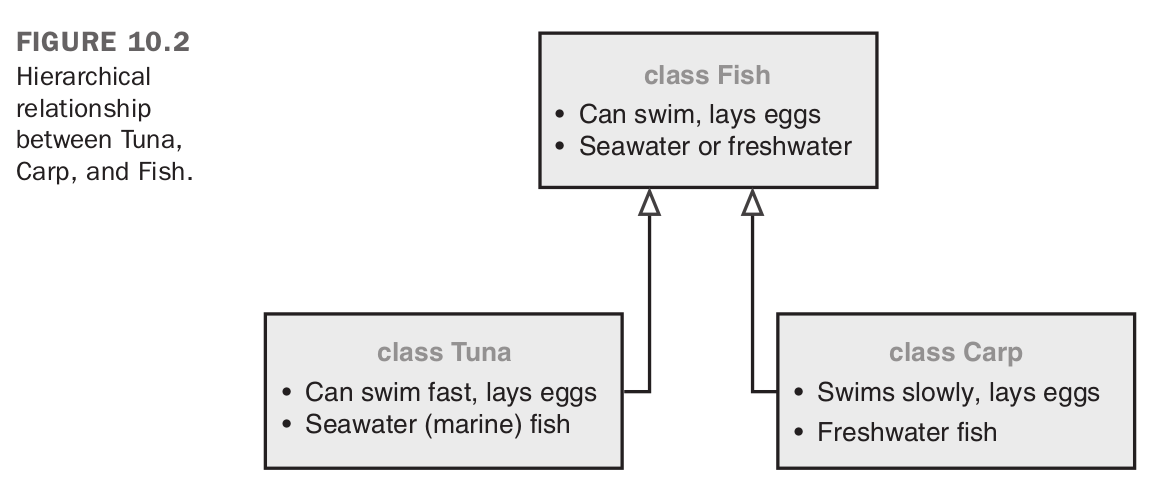
\includegraphics[width=\linewidth]{fishies}
\end{columns}
\end{frame}

\begin{frame}[fragile]{Að skilgreina erfðir}
\begin{columns}
\column{0.5\textwidth}
\begin{itemize}
 \item Þegar klasi $B$ erfir frá $A$ fær $B$ aðgang að aðferðum og eiginleikum $A$
 \item Síðan höfum við val um hversu mikinn aðgang tilvik af $B$ hafa að eiginleikum $A$
 \item Venjulega munum við nota \texttt{public} aðgang
\end{itemize}
\column{0.5\textwidth}
\begin{minted}[frame=lines, fontsize=\small]{cpp}
class A {
  // ... base class members
};
class B: access-specifier A {
  // ... derived class members
};
\end{minted}
\end{columns}
\end{frame}

\begin{frame}[fragile]{Dæmi}
Tvær gerðir af \texttt{Fish} sem eiga það sameiginlegt að geta framkvæmt \texttt{swim()}.
\begin{columns}
\column{0.45\textwidth}
\cppfile[firstline=5, lastline=15, label=fishies.cpp, fontsize=\tiny, linenos=true]{Code/w2/fishies.cpp}
\column{0.45\textwidth}
\cppfile[firstline=17, lastline=22, label=fishies.cpp, fontsize=\tiny, linenos=true]{Code/w2/fishies.cpp}
\cppfile[firstline=24, lastline=29, label=fishies.cpp, fontsize=\tiny, linenos=true]{Code/w2/fishies.cpp}
\end{columns}
\end{frame}

\begin{frame}{Dæmi}
\begin{itemize}
 \item Við getum látið tilvik af undirklösum vinna með aðferðir yfirklasa
 \item Getum ákveðið hvernig aðferðirnar eru bundnar
 \begin{itemize}
  \item Þegar forritið er þýtt (e. \emph{early binding})
  \item Þegar forritið er keyrt og tag hlutarins ljóst (e. \emph{late binding})
 \end{itemize}
 \item Getum tilgreint ``late binding'' með \texttt{virtual} lykilorðinu
 \item Sjá: polymorphismi!
\end{itemize}
\end{frame}

\subsection{Fjölbinding virkja}

\begin{frame}{Fjölbinding}
\begin{itemize}
 \item Við könnumst nú þegar við það að virki geti virkað á mismunandi hátt á mismunandi gögn!
 \begin{itemize}
  \item $1 + 2$ er ekki reiknað á sama hátt og $\frac{2}{3} + \frac{4}{3}$, þó við skiljum aðgerðina á sama hátt
  \item Það sama á við í forritun - samlagning á tveimur \texttt{double} tölum fer ekki eins fram og samlagning á tveimur \texttt{int} tölum
 \end{itemize}
 \item Í C++ getum við skilgreint hvaða merkingu virki á að hafa á tilvik klasanna okkar
\end{itemize}
\end{frame}

\begin{frame}{Fjölbinding í C++}
Við getum skilgreint hvernig tvíundarvirkjar (með tvö viðföng) virka á tilvik af klasanum okkar með því að skilgreina nýja aðferð í klasanum:
\begin{center}
\texttt{return\_type operator\_type (parameter);}
\end{center}
Lítum á \texttt{lego.cpp}!
\end{frame}

\section{Lokaorð}

\begin{frame}{Merkilegri klasar}
\begin{itemize}
 \item Skólabókardæmi um klasa/hluti líkja oft eftir efnislegum hlutum
 \begin{itemize}
  \item Frekar klént
 \end{itemize}
 \item Hlutbundin aðferðafræði er þó iðulega notuð um ``hluti'' sem samsvara ekki neinum hlutum sem hægt væri að snerta
 \begin{itemize}
  \item \texttt{DatabaseConnection}, \texttt{ResourceManager}, \texttt{JSONEncoder}, \ldots
 \end{itemize}
 \item Munum nota hlutbundna forritun til að útfæra ýmsar gagnagrindur
\end{itemize}
\end{frame}

\begin{frame}{Þessi glærupakki}
Tengill á fyrirlestraræfingu: \url{https://goo.gl/forms/CtaT9EV2f9xjpEC92}
\vspace{1cm}

Öll nafngreind forrit í þessum glærupakka, ásamt glærupakkanum sjálfum, má finna á  \href{https://github.com/Ernir/kennsluefni/tree/master/T2/Code/w2}{Github}.
\end{frame}


\begin{frame}{Næst}
Staðalsafn C++
\end{frame}


\end{document}
